\documentclass[english,openright ,hidelinks,pdftex, 11 pt, class=article,crop=false]{standalone}

\usepackage[utf8]{luainputenc}
\usepackage{geometry}
\geometry{verbose,paperwidth=16.4 cm, paperheight=23 cm, inner=2.05cm, outer=2.05 cm, bmargin=2cm, tmargin=1.8cm}
\setlength{\parindent}{0bp}
\usepackage{import}
\usepackage[subpreambles=false]{standalone}
\usepackage{amsmath}
\usepackage{amssymb}
\usepackage{esint}
\usepackage{babel}
\makeatletter
\makeatother
\usepackage{babel}
\usepackage{graphicx}
\usepackage{float}
\usepackage{subfig}
\usepackage[dvipsnames]{xcolor}
\usepackage[many]{tcolorbox}
\newcommand\eks[2][]{\begin{tcolorbox}[boxrule=0.3 mm,arc=0mm,enhanced jigsaw,breakable,colback=green!15] {\large \textbf{Eksempel #1} \vspace{5 pt}\\} #2 \end{tcolorbox}\vspace{-5pt} }
\begin{document}
\section*{Oppgave 1}
\thispagestyle{empty}
Teikn inn og finn svara på gongestykka. \\[11pt]

\eks{
	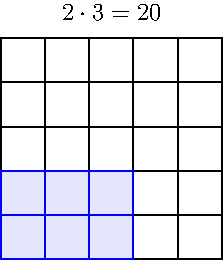
\includegraphics[]{opg1a}
\hfill

\includegraphics[]{opg1b}
}
\vspace{20pt}
	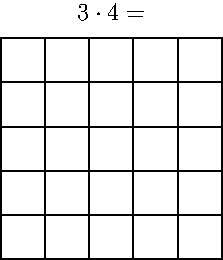
\includegraphics[]{opg1c}
\hfill
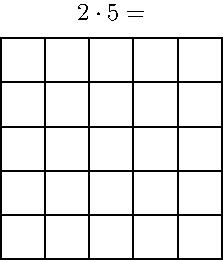
\includegraphics[]{opg1d}

\vspace{20pt}
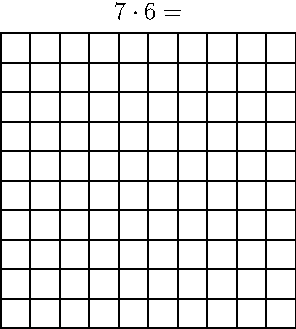
\includegraphics[]{opg1e}
\hfill
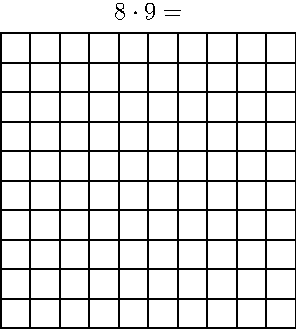
\includegraphics[]{opg1f}
\end{document}